\chapter{Diseño e implementación}

\label{Chapter3}

Este capítulo detalla la arquitectura del prototipo de telemetría, el diseño del hardware, la implementación de la comunicación con los periféricos y la integración con el dispositivo móvil.

El capítulo se organiza en cinco ejes alineados con la estructura del proyecto. En primer lugar se describe la arquitectura del sistema y el uso de la memoria del integrado. En segundo lugar se presenta el diseño del hardware del prototipo. En tercer lugar se documenta el diseño del firmware embebido y sus módulos principales. En cuarto lugar se describen las interfaces de comunicación y el formato de los mensajes intercambiados. Por último se explica la integración con la aplicación web en el teléfono.

%----------------------------------------------------------------------------------------
\section{Arquitectura del sistema}
\label{sec:arquitectura-sistema}

La arquitectura del prototipo se presenta en un recorrido de cuatro pasos encadenados. La figura~\ref{fig:arquitectura-dos-partes-cap3} sitúa primero las dos partes del sistema y el tipo de acoplamiento entre ellas. La figura~\ref{fig:interconexion-buses-cap3} detalla el lado embebido como bloques cableados al microcontrolador. La figura~\ref{fig:capas-software-cap3} contrasta a continuación las capas de software en el integrado y en el teléfono. El recorrido cierra con el uso de la memoria interna del integrado, donde residieron el firmware y los datos activos durante la ejecución.

Tal como resume la figura~\ref{fig:arquitectura-dos-partes-cap3}, el dispositivo embebido en la motocicleta adquirió datos inerciales y de posicionamiento, registró series temporales en almacenamiento local y expuso un enlace serie hacia un módulo BLE. El teléfono móvil concentró la interfaz de usuario, la visualización cartográfica y la recepción de telemetría cuando existió emparejamiento inalámbrico. Esa distribución, de acoplamiento flexible, preservó el registro autónomo aun si el conductor no abrió la aplicación web.

\begin{figure}[H]
	\centering
	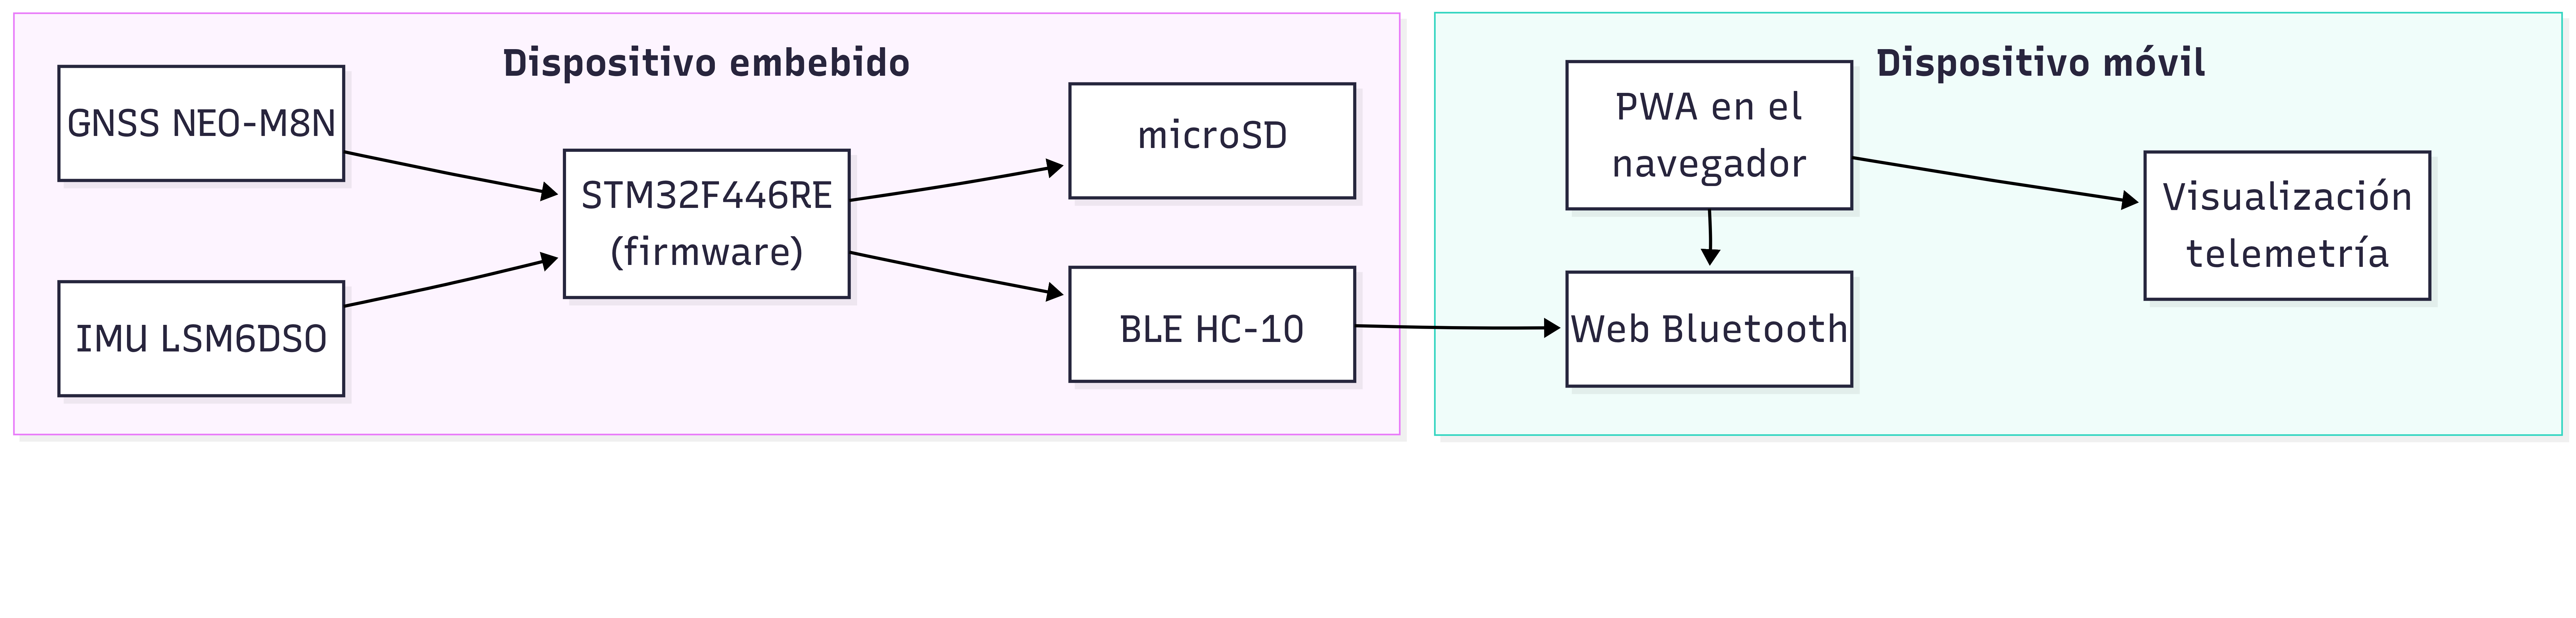
\includegraphics[width=0.95\textwidth]{Figures/arquitectura-dos-partes.png}
	\caption[Arquitectura en dos partes]{Arquitectura general del sistema: dispositivo embebido y dispositivo móvil.}
	\label{fig:arquitectura-dos-partes-cap3}
\end{figure}

La figura anterior fija roles y flujos de información entre el vehículo y el teléfono. El resto de esta sección baja de nivel y desglosa primero el hardware lógico del bloque embebido, luego el software en ambos extremos y, al final, los recursos de memoria del integrado.

\subsection{Interconexión de módulos}

En el dispositivo embebido del prototipo el procesamiento se concentró en el microcontrolador STM32F446RE de la placa NUCLEO-F446RE \citep{st_nucleo_f446re}. A ese integrado se cablearon el receptor GNSS NEO-M8N, la unidad inercial LSM6DSO, el módulo de enlace Bluetooth HC-10 y el slot de tarjeta microSD, en correspondencia con los bloques del diagrama de dos partes. La figura~\ref{fig:interconexion-buses-cap3} resume la interconexión lógica entre el microcontrolador y esos periféricos.

\begin{figure}[H]
	\centering
	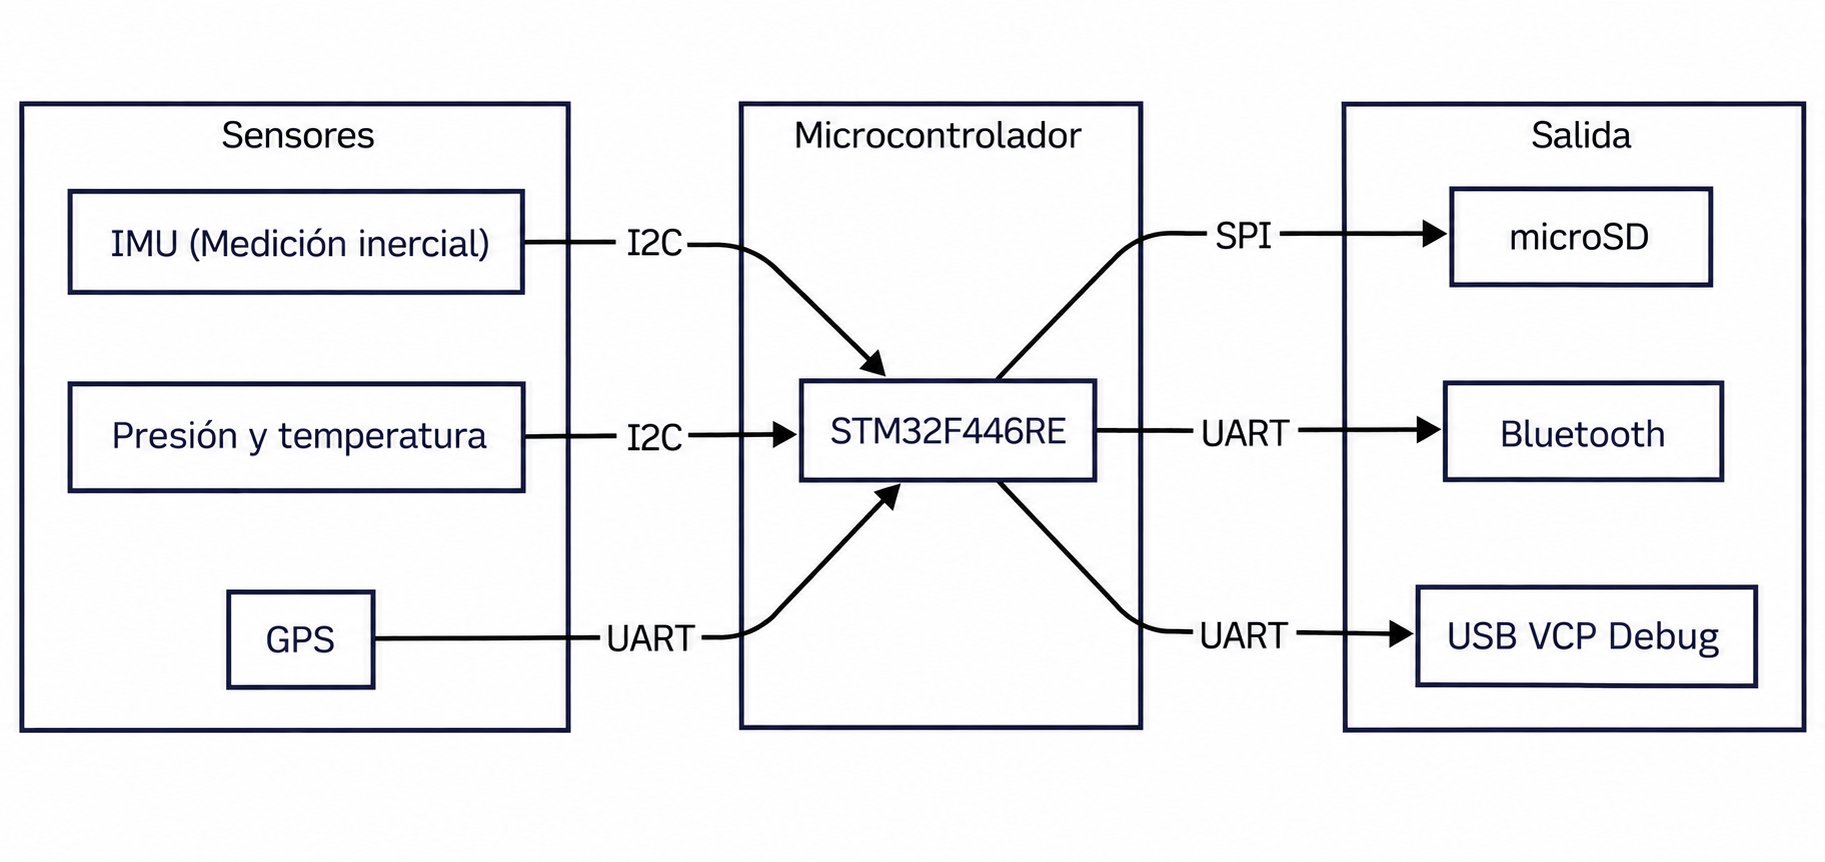
\includegraphics[width=0.92\textwidth]{Figures/interconexion-buses.png}
	\caption[Arquitectura en bloques]{Diagrama en bloques de la interconexión entre el microcontrolador y los periféricos del prototipo.}
	\label{fig:interconexion-buses-cap3}
\end{figure}

Cada módulo utilizó el bus serie indicado en el diagrama: NEO-M8N por USART1, LSM6DSO por I2C1, HC-10 por USART3 y microSD por SPI2. La tabla~\ref{tab:parametros-buses} de la sección~\ref{sec:comunicaciones-implementacion} explica en detalle instancias, velocidades y rol de cada enlace en el firmware. Las secciones~\ref{sec:diseno-hardware} y~\ref{sec:comunicaciones-implementacion} desarrollan el cableado físico y el comportamiento de cada interfaz.

\subsection{Arquitectura de software}

Con la interconexión de módulos definida, el software repartió las mismas funciones entre capas en el microcontrolador y en el teléfono. En el integrado intervinieron la HAL, controladores para el GPS, la unidad inercial, el enlace Bluetooth y el manejo de la tarjeta microSD, además del middleware FatFs \citep{chan_fatfs}. Sobre esa base se empleó el sistema operativo de tiempo real FreeRTOS \citep{freertos}. Las tareas del planificador actuaron como objetos activos del firmware, cada una con una responsabilidad acotada y una prioridad de ejecución. Las colas intercambiaron muestras y eventos entre la adquisición, el registro en tarjeta y el enlace Bluetooth. Los semáforos indicaron cuándo había tramas GNSS o lecturas inerciales listas para procesar. El mutex reservó de forma exclusiva el bus SPI ante accesos concurrentes a la microSD. Con ese esquema coexistieron en paralelo la adquisición de sensores, el registro local y la publicación por Bluetooth. El acceso al hardware quedó mediado por drivers y por transferencias DMA en los enlaces de mayor caudal. En el teléfono, la PWA usó el Bluetooth del navegador \citep{mdn_pwa}\citep{w3c_web_bluetooth} para conectarse al dispositivo embebido y recibir telemetría. La figura~\ref{fig:capas-software-cap3} contrasta ambos lados del sistema.

\begin{figure}[H]
	\centering
	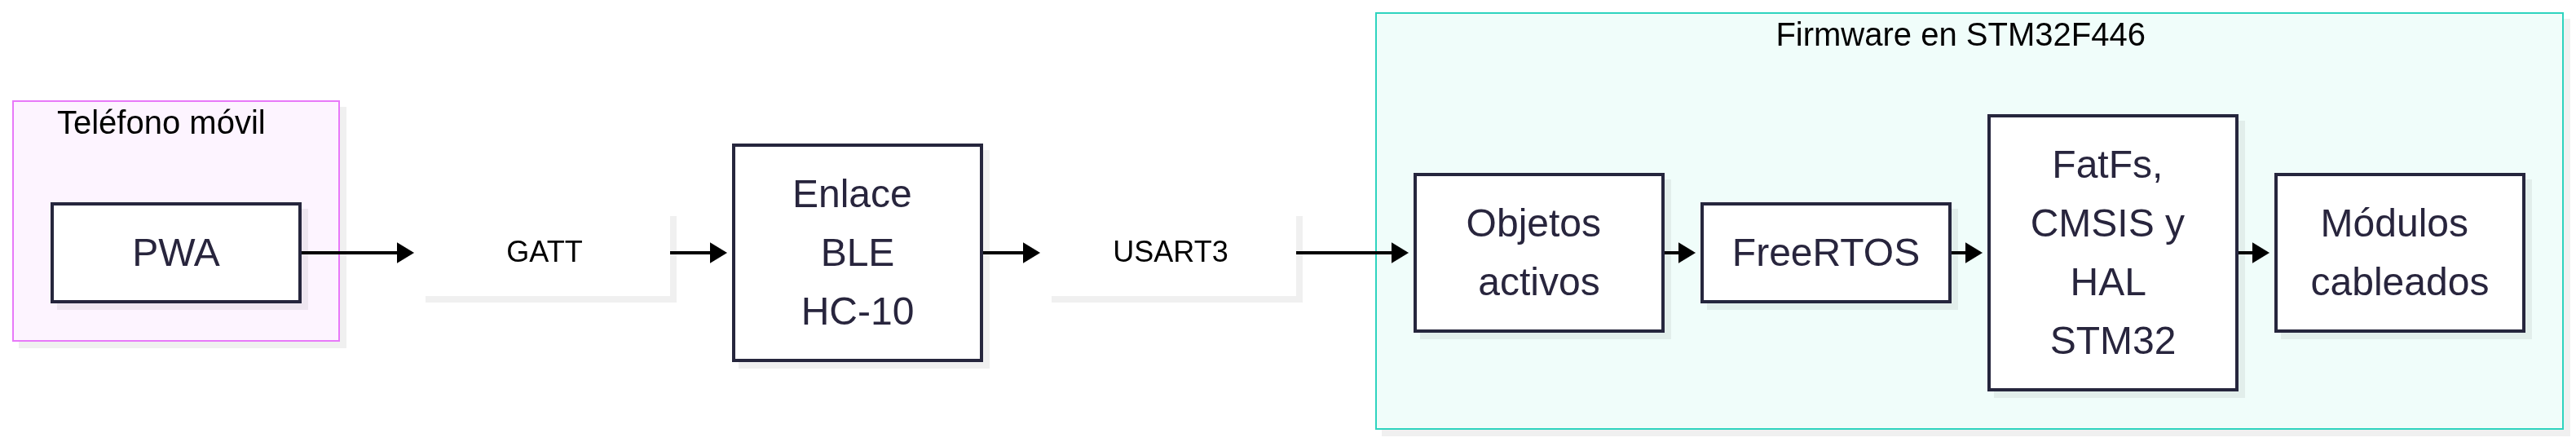
\includegraphics[width=0.95\textwidth]{Figures/cap2-capas-software.png}
	\caption[Capas de software]{Capas de software en el microcontrolador y en el teléfono móvil.}
	\label{fig:capas-software-cap3}
\end{figure}

Las capas del diagrama anterior condicionan el uso de memoria y el reparto de tareas descrito en la sección~\ref{sec:diseno-firmware}. A continuación se resume dónde reside el programa embarcado y las estructuras de datos en tiempo de ejecución.

\subsection{Uso de la memoria del integrado}
\label{sec:modelo-memoria-mcu}

El código del firmware residió en la memoria flash interna. En la SRAM se ubicaron las pilas de las tareas del RTOS, los buffers de DMA, las colas de mensajes y las estructuras de telemetría. Entre estos últimos encajaron el estado de los controladores, el búfer circular del GNSS y las áreas de trabajo que FatFs empleó durante las escrituras en la tarjeta. Todo ello permaneció acotado a los 512KiB de flash y los 128KiB de SRAM del STM32F446RET6, sin memoria de programa ni RAM externas. La descripción de pines, relojes, instancias de DMA y periféricos se generó con STM32CubeMX y se integró al proyecto en STM32CubeIDE \citep{st_stm32cubeide}. El IWDG se habilitó como una supervisión ante bloqueos del software y se alimentó de forma periódica desde una tarea dedicada del RTOS.

%----------------------------------------------------------------------------------------
\section{Diseño del hardware}
\label{sec:diseno-hardware}

Tras la vista lógica de la sección~\ref{sec:arquitectura-sistema}, esta sección traduce los mismos bloques a un diseño eléctrico y a un circuito impreso apto para montar en el vehículo. En primer lugar se presenta el esquemático. En segundo lugar se muestra el PCB que integra conectores, alimentación y rutas hacia los periféricos del diagrama en bloques.

\subsection{Esquema eléctrico}

El esquema reunió el microcontrolador, la alimentación, los conectores hacia GNSS, la unidad inercial, la tarjeta microSD y el módulo de enlace Bluetooth, con la misma asignación lógica de buses que resume la figura~\ref{fig:interconexion-buses-cap3}. La figura~\ref{fig:cap3-esquema-electrico} muestra el diagrama eléctrico del prototipo.

\begin{figure}[H]
	\centering
	\fbox{\begin{minipage}{0.9\textwidth}
		\centering\vspace{0.28\textheight}
		\textit{Espacio reservado para el esquema eléctrico.}\vspace{0.28\textheight}
	\end{minipage}}
	\caption[Esquema eléctrico]{Esquema eléctrico del prototipo de telemetría.}
	\label{fig:cap3-esquema-electrico}
\end{figure}

\subsection{Circuito impreso}

El circuito impreso integró los bloques del esquema en un único PCB orientado al montaje en el vehículo. La figura~\ref{fig:cap3-pcb} presenta el diseño de la placa (vista superior o de ensamblado).

\begin{figure}[H]
	\centering
	\fbox{\begin{minipage}{0.9\textwidth}
		\centering\vspace{0.28\textheight}
		\textit{Espacio reservado para el diseño del circuito impreso.}\vspace{0.28\textheight}
	\end{minipage}}
	\caption[Circuito impreso]{Vista del circuito impreso del prototipo.}
	\label{fig:cap3-pcb}
\end{figure}

%----------------------------------------------------------------------------------------
\section{Diseño del firmware}
\label{sec:diseno-firmware}

El firmware implementó las funciones del dispositivo embebido descritas en la sección~\ref{sec:arquitectura-sistema}. Coordinó adquisición, registro local y el enlace Bluetooth mediante controladores por periférico y tareas del RTOS. La subsección siguiente detalla esa organización modular y el reparto de actividades.

\subsection{Organización en módulos}

La lógica embebida se repartió en controladores que encapsulan cada periférico y en tareas de FreeRTOS que orquestan el muestreo y la publicación de datos. Los módulos \texttt{gps} y \texttt{lsm6dso} abstraen la lectura de GNSS y de la IMU. El módulo \texttt{bt\_module} concentra el envío por USART3. El módulo \texttt{sd\_logger}, junto con FatFs, administra el fichero CSV en la tarjeta microSD. Esos controladores concentraron el acceso al hardware, mientras que las tareas del planificador actuaron como objetos activos: cada una ejecutó un ciclo de trabajo propio, con prioridad asignada, y entregó datos al resto del firmware mediante colas y señales del kernel.

Tras la inicialización del hardware y el arranque del planificador del sistema operativo de tiempo real, coexistieron objetos activos dedicados a la adquisición y análisis de NMEA, la lectura periódica de la IMU, el registro en la tarjeta microSD y el enlace Bluetooth. Las tareas que acceden al bus SPI de la tarjeta serializaron el acceso al medio mediante un mutex (del inglés \textit{mutual exclusion}) del RTOS para evitar corrupción de ficheros. Los eventos entre módulos se canalizaron con colas y temporizadores de software del kernel. La figura~\ref{fig:cap3-flujo-firmware} resume el encadenamiento desde el periférico hasta las estructuras de telemetría y el resto de objetos activos. En ella se representa el flujo de la IMU (LSM6DSO) como ejemplo ilustrativo del patrón. En el firmware se repitió la misma lógica de controlador, tarea y colas con el GNSS, el registro en microSD y el enlace Bluetooth.

El IWDG del microcontrolador se habilitó en el arranque como supervisión ante bloqueos del software. Una tarea dedicada del RTOS ejecutó un ciclo periódico que refrescó el contador del watchdog independiente antes de que venciera el margen configurado. Si una falla impidió esa actualización, el hardware reinició el MCU y el firmware volvió a iniciar la adquisición y el registro sin intervención manual. Esa capa complementó el reparto de prioridades del planificador y redujo el riesgo de dejar el prototipo inoperante en marcha.

\begin{figure}[H]
	\centering
	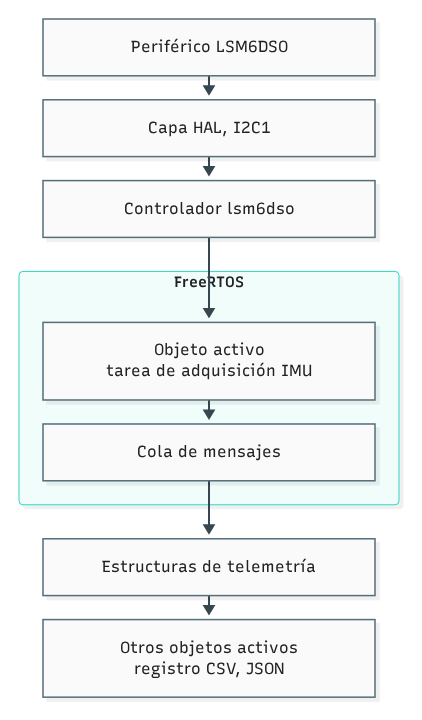
\includegraphics[width=0.52\textwidth]{Figures/cap3-flujo-firmware.png}
	\caption[Flujo del firmware]{Encadenamiento periférico, controlador, RTOS y telemetría.}
	\label{fig:cap3-flujo-firmware}
\end{figure}

%----------------------------------------------------------------------------------------
\section{Comunicaciones e interfaces}
\label{sec:comunicaciones-implementacion}

Esta sección documenta cómo se enlazaron los buses del microcontrolador con cada módulo, qué mensajes intercambiaron el firmware y el teléfono, y qué canal quedó previsto para depuración. En primer lugar se resume la asignación de instancias USART, I2C y SPI. En segundo lugar se describe el protocolo de telemetría en \texttt{JSON} sobre el enlace Bluetooth. Por último se describe el puerto serie de depuración.

\subsection{Asignación de periféricos}

En el STM32F446RE se configuró qué instancia de cada bus (USART, I2C y SPI) enlazó a cada módulo del prototipo. STM32CubeMX fijó también los pines y la velocidad de cada enlace. La tabla~\ref{tab:parametros-buses} resume esa asignación, el modo de operación y el rol de cada enlace en el firmware.

\begin{table}[H]
	\centering
	\caption[Parámetros de buses]{Parámetros de los buses configurados en el prototipo.}
	\setlength{\tabcolsep}{4pt}
	\begin{tabularx}{\textwidth}{@{}>{\raggedright\arraybackslash}p{1.45cm}>{\raggedright\arraybackslash}p{1.95cm}>{\raggedright\arraybackslash}p{2.35cm}>{\raggedright\arraybackslash}X@{}}
		\toprule
		\textbf{Bus} & \textbf{Periférico} & \textbf{Tasa / modo} & \textbf{Rol en el sistema} \\
		\midrule
		USART1 & NEO-M8N & 9600 baudios & Recepción NMEA por DMA hacia buffer circular \\
		USART2 & ST-LINK VCP & 115200 baudios & Consola de depuración hacia el host \\
		USART3 & HC-10 (BLE) & 9600 baudios & Enlace serie transparente con el teléfono \\
		I2C1 & LSM6DSO & 100kHz, maestro & Lectura periódica de registros de la IMU \\
		SPI2 & microSD & Maestro, DMA & Almacenamiento de ficheros CSV mediante FatFs \\
		\bottomrule
	\end{tabularx}
	\label{tab:parametros-buses}
\end{table}

La tabla anterior enlaza cada bus con el módulo físico y con la responsabilidad asignada en software. Sobre USART3, el mismo enlace que enlaza al HC-10 según la figura~\ref{fig:interconexion-buses-cap3}, circuló la telemetría hacia el teléfono. El registro en SPI2 permaneció independiente de ese intercambio inalámbrico. El apartado siguiente describe el contenido de la trama de telemetría y su relación con el almacenamiento local.

\subsection{Protocolo de telemetría sobre el enlace serie}
\label{sec:protocolo-telemetria-serie}

En USART1 el canal DMA copió al buffer circular los octetos recibidos por el puerto serie. Una tarea de mayor prioridad reconstruyó las sentencias NMEA \citep{nmea_0183} a partir de ese buffer y, si una línea era válida, se conservó en memoria la posición, la hora y los demás datos de navegación que aportaba. Las líneas incompletas o incorrectas se descartaron. En I2C1 la unidad inercial se consultó en modo maestro a 100kHz con dirección de 7 bits 0x6A desde la tarea de adquisición.

En USART3 el módulo HC-10 funcionó como túnel serie hacia el teléfono. El microcontrolador envió octetos por UART y el módulo los reexpuso por BLE para que el navegador móvil los recibiera. Una tarea de enlace publicó la telemetría en formato \texttt{JSON}. Cada ciclo emitió una única trama, una línea de texto por muestra, que reunió en un mismo objeto las magnitudes inerciales y las de posicionamiento. La trama incluyó aceleraciones y velocidades angulares en los tres ejes, temperatura de la IMU con enteros escalados, tipo de fijación GNSS derivado de las sentencias NMEA \citep{nmea_0183} (sin posición, fijación en dos dimensiones, fijación en tres dimensiones con altitud o fijación con corrección diferencial), coordenadas geográficas, altitud, velocidad sobre el suelo, cantidad de satélites en uso y rumbo. No se definió un protocolo binario propietario sobre el UART.

En SPI2 las transferencias en bloque hacia la tarjeta se realizaron con DMA bajo FatFs para reducir la carga del núcleo durante la escritura del fichero CSV. Cada registro incluyó una marca temporal en milisegundos, la hora UTC cuando el receptor GNSS dispuso de fecha y hora válidas, las tres componentes de aceleración y de velocidad angular, y la temperatura de la IMU. La primera fila del archivo declaró las columnas correspondientes y las sucesivas se alinearon al período de muestreo configurado en el firmware.

La figura~\ref{fig:cap3-formato-mensaje} representa la organización de la trama \texttt{JSON}. La figura~\ref{fig:cap3-secuencia-comunicacion} ilustra la secuencia entre el ciclo de telemetría, el módulo HC-10 y el dispositivo móvil.

\begin{figure}[H]
	\centering
	\fbox{\begin{minipage}{0.88\textwidth}
		\centering\vspace{0.22\textheight}
		\textit{Espacio reservado para organización de la trama JSON de telemetría.}\vspace{0.22\textheight}
	\end{minipage}}
	\caption[Organización de la trama]{Organización de los campos en la trama JSON de telemetría.}
	\label{fig:cap3-formato-mensaje}
\end{figure}

\begin{figure}[H]
	\centering
	\fbox{\begin{minipage}{0.88\textwidth}
		\centering\vspace{0.30\textheight}
		\textit{Espacio reservado para diagrama de secuencia de comunicación.}\vspace{0.30\textheight}
	\end{minipage}}
	\caption[Secuencia de comunicación]{Diagrama de secuencia del intercambio entre firmware, HC-10 y dispositivo móvil.}
	\label{fig:cap3-secuencia-comunicacion}
\end{figure}

\subsection{Canal de depuración}

USART2 enlazó al puerto virtual del depurador ST-LINK. El diseño previó un canal opcional de trazas por ese enlace, activable o desactivable al compilar el firmware, separado de la telemetría \texttt{JSON} hacia el teléfono y del registro en microSD. Los ensayos que ejercitaron ese canal y el análisis de los mensajes emitidos se documentan en el capítulo~\ref{Chapter4}.

%----------------------------------------------------------------------------------------
\section{Integración entre hardware y software}
\label{sec:integracion-hw-sw}

El prototipo se cerró con la aplicación en el teléfono y con el recorrido de los datos desde los sensores hasta la visualización. Esta sección resume el software del dispositivo móvil y describe el flujo extremo a extremo que une registro local, enlace inalámbrico e interfaz de usuario.

\subsection{Dispositivo móvil}
\label{sec:dispositivo-movil}

La interfaz del usuario se desarrolló como una aplicación web progresiva (PWA) con React \citep{react} y Vite \citep{vite}, accesible desde el navegador sin publicar un binario en las tiendas de aplicaciones. El enlace con el prototipo embebido reutilizó el mismo flujo \texttt{JSON} descrito en la sección~\ref{sec:protocolo-telemetria-serie}. En el teléfono las tramas atravesaron la pila BLE del módulo HC-10 antes de alimentar la capa de presentación.

En el navegador compatible se empleó la API Web Bluetooth \citep{w3c_web_bluetooth} para emparejar el HC-10. La selección del periférico filtró por el servicio GATT (del inglés \textit{Generic Attribute Profile}) de tipo UART del BT05, con identificador 0xFFE0, y por el prefijo habitual del nombre visible en el escaneo. Tras abrir la conexión GATT con el CC2541, la aplicación accedió al servicio primario 0xFFE0 y suscribió notificaciones sobre la característica 0xFFE1, que el módulo asocia al puerto serie transparente hacia el STM32.

Cada notificación entregó un fragmento de octetos que la capa de lectura decodificó como texto UTF-8 y acumuló en un búfer de líneas. El separador de fin de línea partió los fragmentos hasta reconstruir tramas completas, de forma análoga al ensamblado de sentencias NMEA en el firmware. Las líneas que comenzaban con llave se interpretaron como la trama única de telemetría en \texttt{JSON} y se validaron los campos previstos antes de incorporar la muestra al estado de la aplicación. Las tramas mal formadas se descartaron sin interrumpir la sesión.

Cada trama válida actualizó un estado central de telemetría que reunió en la misma muestra datos inerciales y de posicionamiento. Los componentes de la interfaz consumieron ese estado para mostrar magnitudes inerciales, velocidad y rumbo. La capa de mapas con Leaflet \citep{leaflet} proyectó las posiciones válidas y el trazado del recorrido a medida que llegaron nuevos puntos. El procesamiento quedó en el navegador y liberó carga en el microcontrolador.

\begin{figure}[H]
	\centering
	\fbox{\begin{minipage}{0.36\textwidth}
		\centering\vspace{0.34\textheight}
		\textit{Espacio reservado para vista conceptual de la interfaz de usuario en el dispositivo móvil.}\vspace{0.34\textheight}
	\end{minipage}}
	\caption[Interfaz en el móvil]{Vista conceptual de la interfaz de usuario de la PWA en el dispositivo móvil.}
	\label{fig:cap3-ui-movil}
\end{figure}

La figura~\ref{fig:cap3-ui-movil} representa una vista conceptual de esa interfaz en el teléfono.

\subsection{Flujo de datos extremo a extremo}

Las tareas de adquisición actualizaron en paralelo las estructuras de telemetría a partir del GNSS y de la IMU. Una tarea de registro volcó esas muestras al fichero CSV en la microSD de forma periódica, de modo que el historial persistiera aun sin teléfono emparejado. Otra tarea formateó esa información en una única trama \texttt{JSON} por ciclo y la envió por USART3 al módulo HC-10 cuando el enlace Bluetooth estuvo activo.

En el teléfono, con el enlace Bluetooth activo, la PWA aplicó el procedimiento de la sección~\ref{sec:dispositivo-movil} y tradujo los reportes de posición ya parseados en coordenadas sobre el plano cartográfico. La figura~\ref{fig:cap3-integracion-e2e} resume esa cadena desde los sensores hasta la visualización.

\begin{figure}[H]
	\centering
	\fbox{\begin{minipage}{0.88\textwidth}
		\centering\vspace{0.30\textheight}
		\textit{Espacio reservado para diagrama de integración extremo a extremo.}\vspace{0.30\textheight}
	\end{minipage}}
	\caption[Integración extremo a extremo]{Flujo de datos entre sensores, almacenamiento local y dispositivo móvil.}
	\label{fig:cap3-integracion-e2e}
\end{figure}